\section{Тестрование}

В качестве теста для оценки производительности myfs выбран бенчмарк
mdtest~\cite{MDTEST}. Бенчмарк mdtest направлен на тестирование
производительности работы с метаданными в файловой системе. Выбор обусловлен
тем, что в myfs не реализована эффективная работа с большими файлами, поэтому
измерять производительность файлового ввода/вывода нет смысла.


\subsection{Описание тестового окружения}

Тестовое окружение состоит из двухядерного процессора Intel® Core™ i5-6200U
2.30GHz с поддержкой технологии Hyper-Threading (2 потока на ядро), 8GB RAM.
В качестве диска используется Intel SSDSCKKF256H6 540-Series 256Gb SATA-III M.2 
80mm TLC SSD с установленной на нем файловой системой ext4. Система управляется
операционной системой Ubuntu 16.04 LTS с ядром Linux версии
4.12.0-rc1-next-20170519.

В тестах участвуют файловые системы zfs, btrfs, ext4 и myfs. Все файловые
системы кроме myfs используют в качестве диска фиктивное блочное устройство
loop, которое в качестве хранилища использует файл размером 20 Gb в файловой
системе ext4.

Файловая система myfs не использует фиктивное блочное устройство loop, а вместо
этого напрямую использует файл. Дополнительно, чтобы оценить влияние фиктивного
блочного устройства loop проводятся тесты с использованием нативной файловой
системы ext4.

На графиках далее используются следующие обозначения:
\begin{itemize}
  \item myfs-fuse - файловая система myfs на основе библиотеки fuse,
        использующая файл в файловой системе ext4 в качестве хранилища;
  \item ext4-native - файловая система ext4 с настройками по-умолчанию,
        использующая настоящее блочное устройство в качестве хранилища;
  \item ext4-loop - файловая система ext4 с настройками по-умолчанию,
        использующая фиктивное блочное устройство loop в качестве хранилища;
  \item btrfs-loop - файловая система btrfs с настройками по-умолчанию,
        использующая фиктивное блочное устройство loop в качестве хранилища;
  \item zfs-loop - файловая система zfs с настройками по-умолчанию, использующая
        фиктивное блочное устройство loop в качестве хранилища.
\end{itemize}

Бенчмарк mdtest запускается следующей командой:
\begin{lstlisting}[basicstyle=\ttfamily,language=bash]
mpirun -np 8 ./mdtest -n 100000 -i 2 -C -r -u \
       -d <path to mountpoint>
\end{lstlisting}

Опции команды описывают следующее:
\begin{itemize}
  \item -np 8 - говорит, что в тесте участвуют 8 процессов;
  \item -n 100000 - каждый из процессов создает 100000 файлов/каталогов;
  \item -u - каждый из процессов создает для себя уникальный каталог и работает
        в нем;
  \item -i 2 - тест повторяется дважды;
  \item -C - процессы должны создать файлы/каталоги;
  \item -r - процессы должны удалить созданные файлы/каталоги.
\end{itemize}

Таким образом тест проверяет скорость создания и удаления файлов и каталогов.
Тест не проверяет скорость чтения/записи, а также не проверяет скорость
выполнения операции stat. О проверке скорости чтения/записи было сказано выше,
а проверка скорости выполнения команды stat убрана из теста так как, ядро Linux
поддерживает кеш inode в памяти и большинство запросов команды stat будут
удовлетворятся из этого кеша, поэтому эти результаты не представляют большого
интереса в контексте данной работы.


\subsection{Результаты тестирования}

В качестве результатов тестирования будут продемонстрированы следующие метрики:
\begin{itemize}
  \item общее время выполнения теста каждой файловой системой, как интергральная
        характеристика производительности;
  \item скорость создания файлов;
  \item скорость удаления файлов;
  \item скорость создания каталогов;
  \item скорость удаления каталогов.
\end{itemize}


\begin{figure}[H]
  \centering
  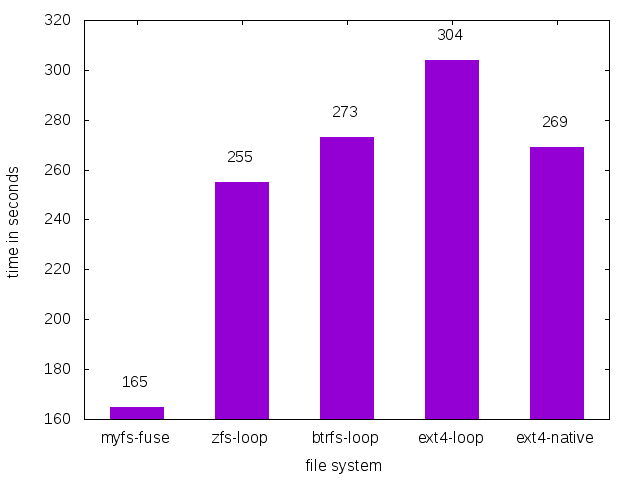
\includegraphics[width=.8\textwidth]{result/total.png}
  \caption{Полное время выполнения теста в секундах}
  \label{pic:total}
\end{figure}

\begin{figure}[H]
  \centering
  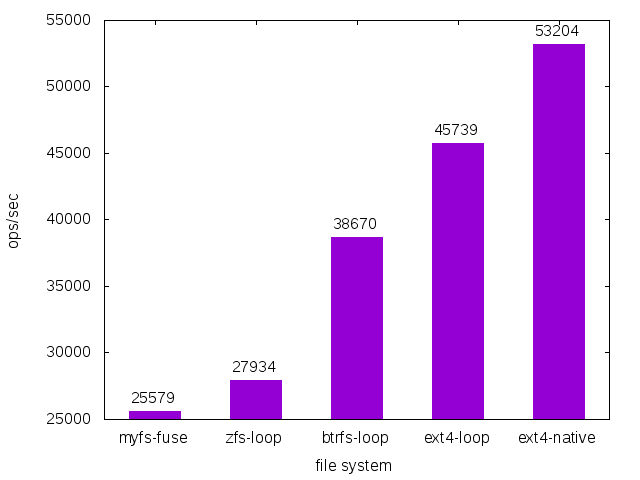
\includegraphics[width=.8\textwidth]{result/fcreat.png}
  \caption{Скорость создания файлов}
  \label{pic:fcreat}
\end{figure}

\begin{figure}[H]
  \centering
  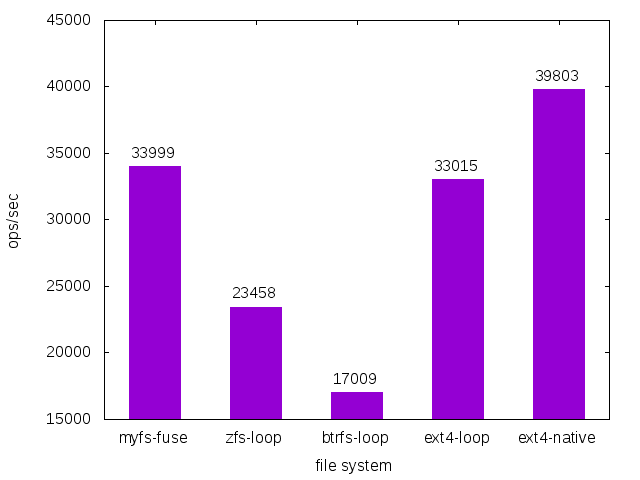
\includegraphics[width=.8\textwidth]{result/fdelet.png}
  \caption{Скорость удаления файлов}
  \label{pic:fdelet}
\end{figure}

\begin{figure}[H]
  \centering
  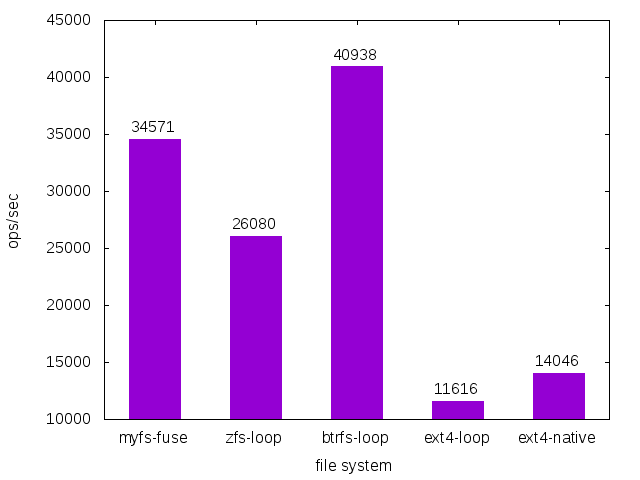
\includegraphics[width=.8\textwidth]{result/dcreat.png}
  \caption{Скорость создания каталогов}
  \label{pic:fdelet}
\end{figure}

\begin{figure}[H]
  \centering
  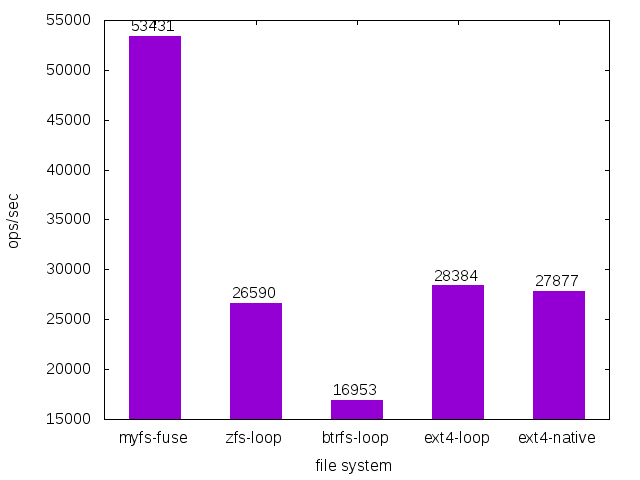
\includegraphics[width=.8\textwidth]{result/ddelet.png}
  \caption{Скорость удаления каталогов}
  \label{pic:fdelet}
\end{figure}
